\documentclass[12pt,a4paper]{article}
\usepackage[utf8]{inputenc}
\usepackage[french]{babel}
\usepackage[T1]{fontenc}
\usepackage{amsmath}
\usepackage{amsfonts}
\usepackage{amssymb}
\usepackage{graphicx}
\author{KONDI Abdoul malik \\ NGANDEU NDJEUKAM Alhasan}
\title{Fiches hebdomadaires : semaine une (1)}
\begin{document}
\maketitle
\tableofcontents
\newpage

\section{Introduction}
	cas d'utilisation
	lll
\section{Ressources}
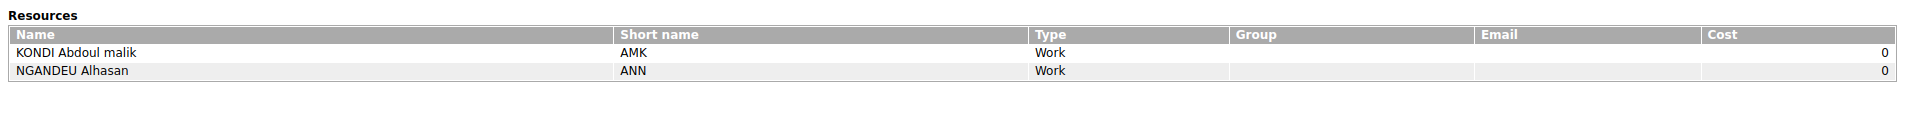
\includegraphics[scale=0.25]{images/resources.png}
\section{Détails des événements passé pendant les cinq (5) jour}
\subsection{Jour 1 : Lundi}

\subsection{Jour 2 : Mardi}
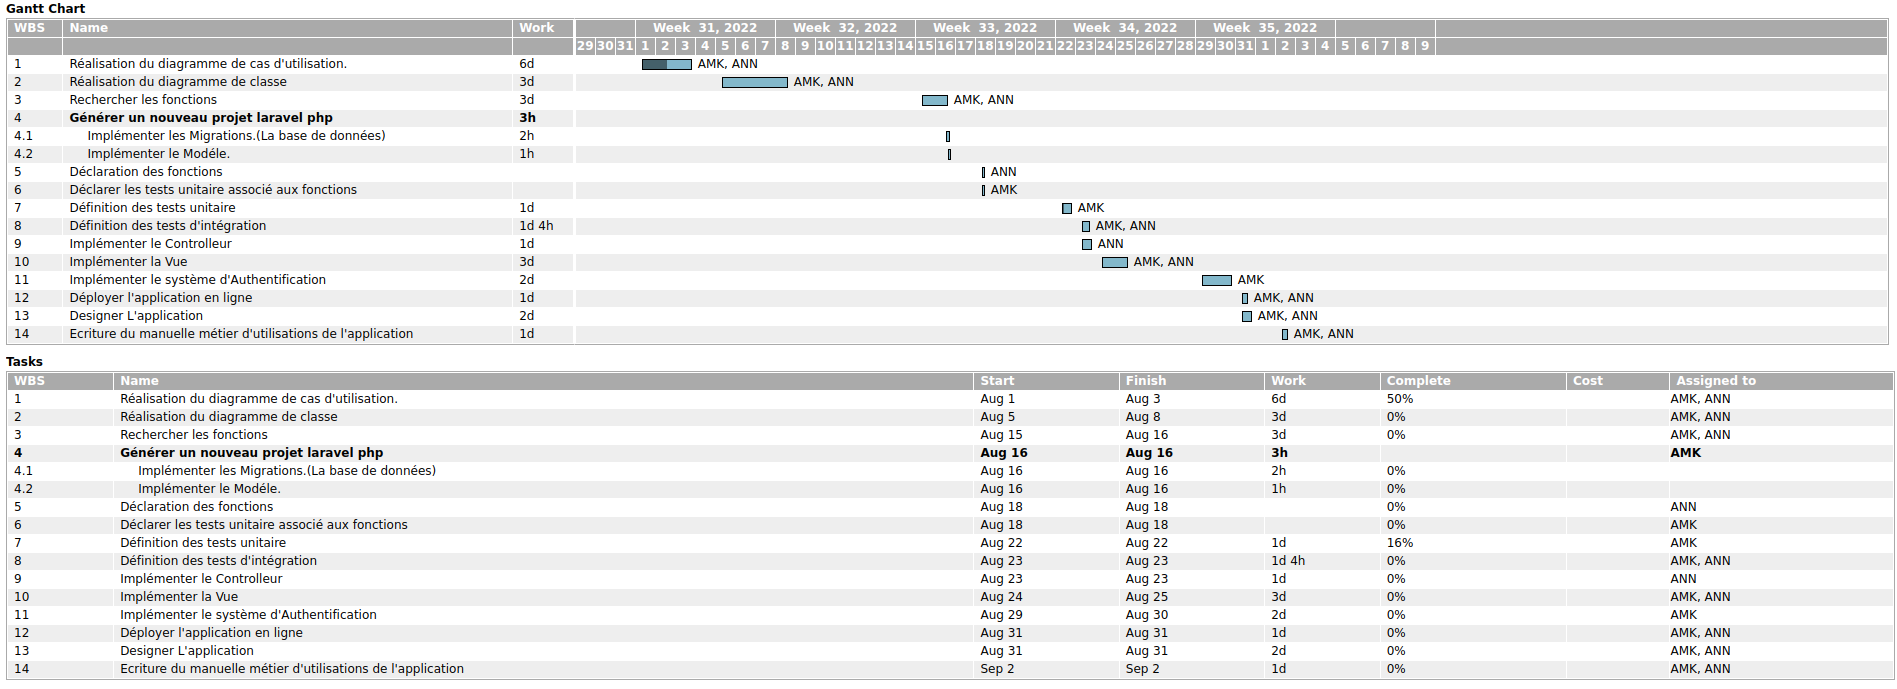
\includegraphics[scale=0.23]{images/jour2.png}
\subsection{Jour 3 : Mercredi}
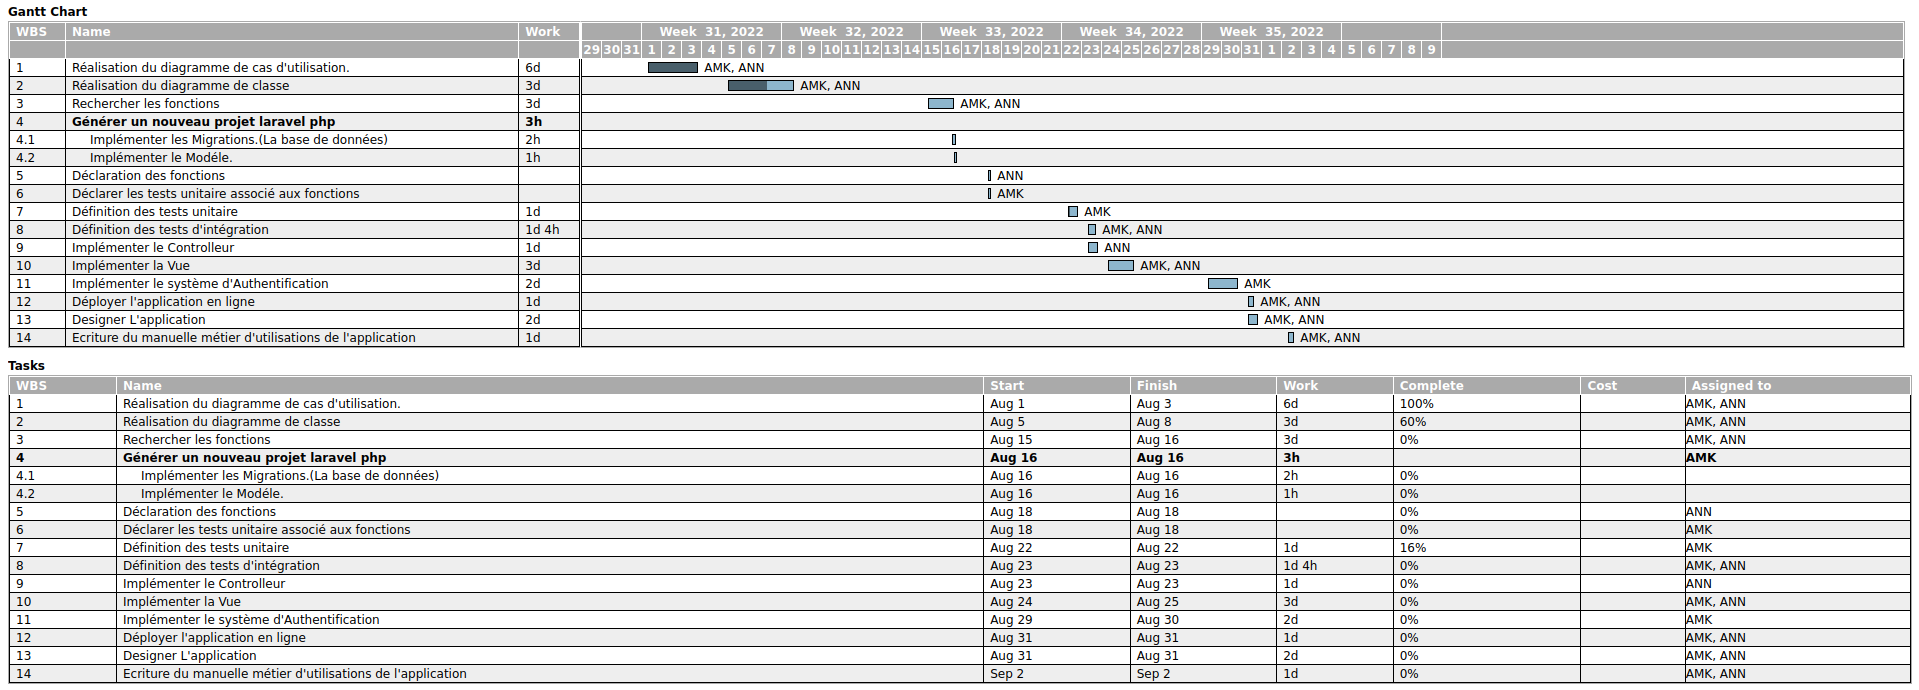
\includegraphics[scale=0.23]{images/jour3.png}
\subsection{Jour 4 : Jeudi}
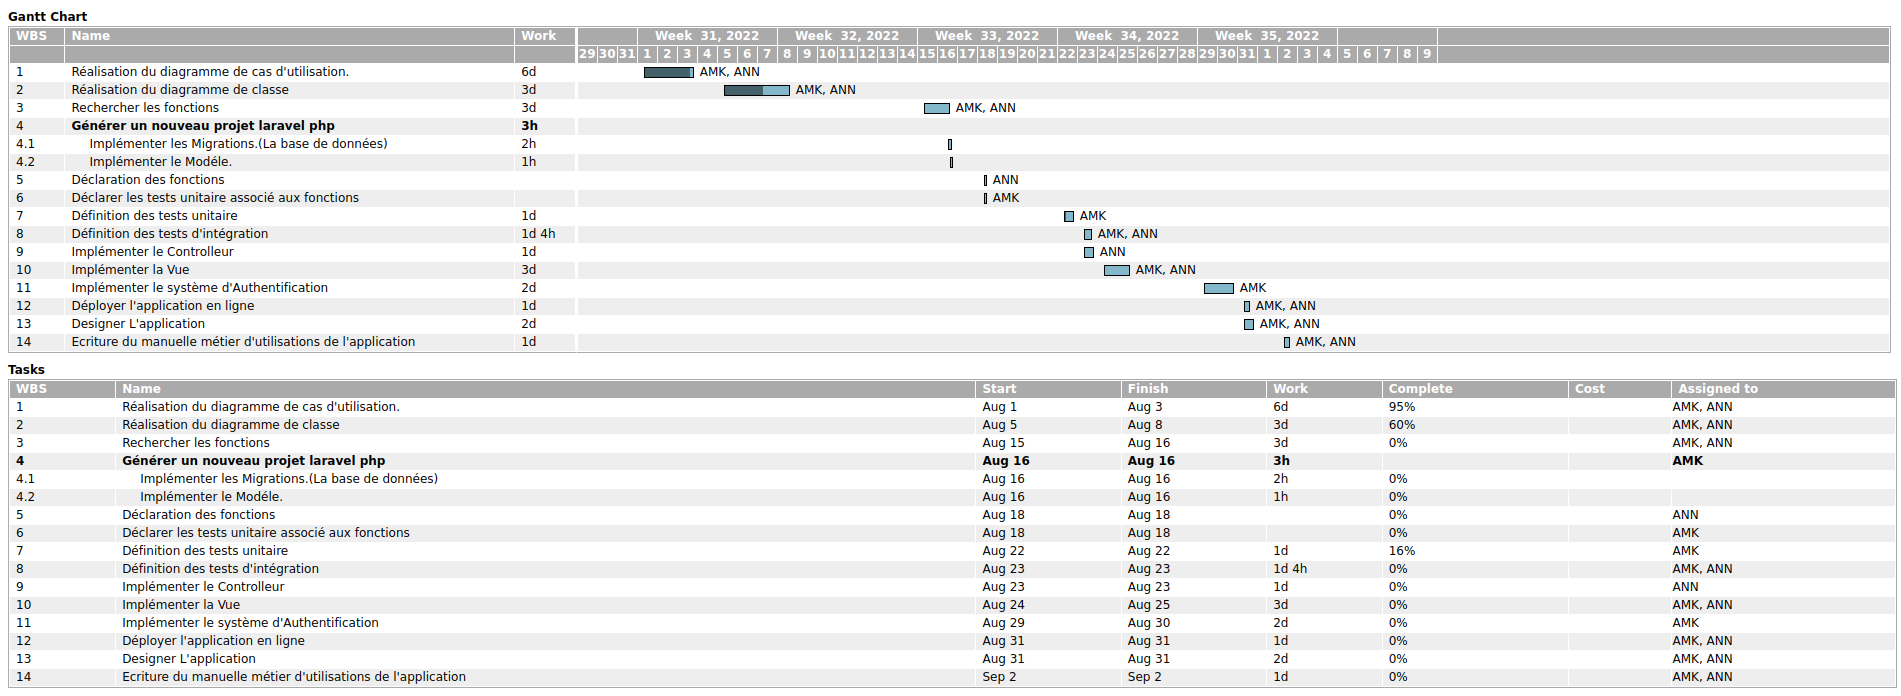
\includegraphics[scale=0.23]{images/jour4.png}
Les activités fait le jeudi sont:
\begin{itemize}
\item Le début de la modélisation du diagramme de classe sous \textbf{modélio}.
\end{itemize}

\textbf{NB:}\\
Le jeudi soir nous n'avons pas pu travailler car malik était tombé malade.

\subsection{Jour 5 : Vendredi}
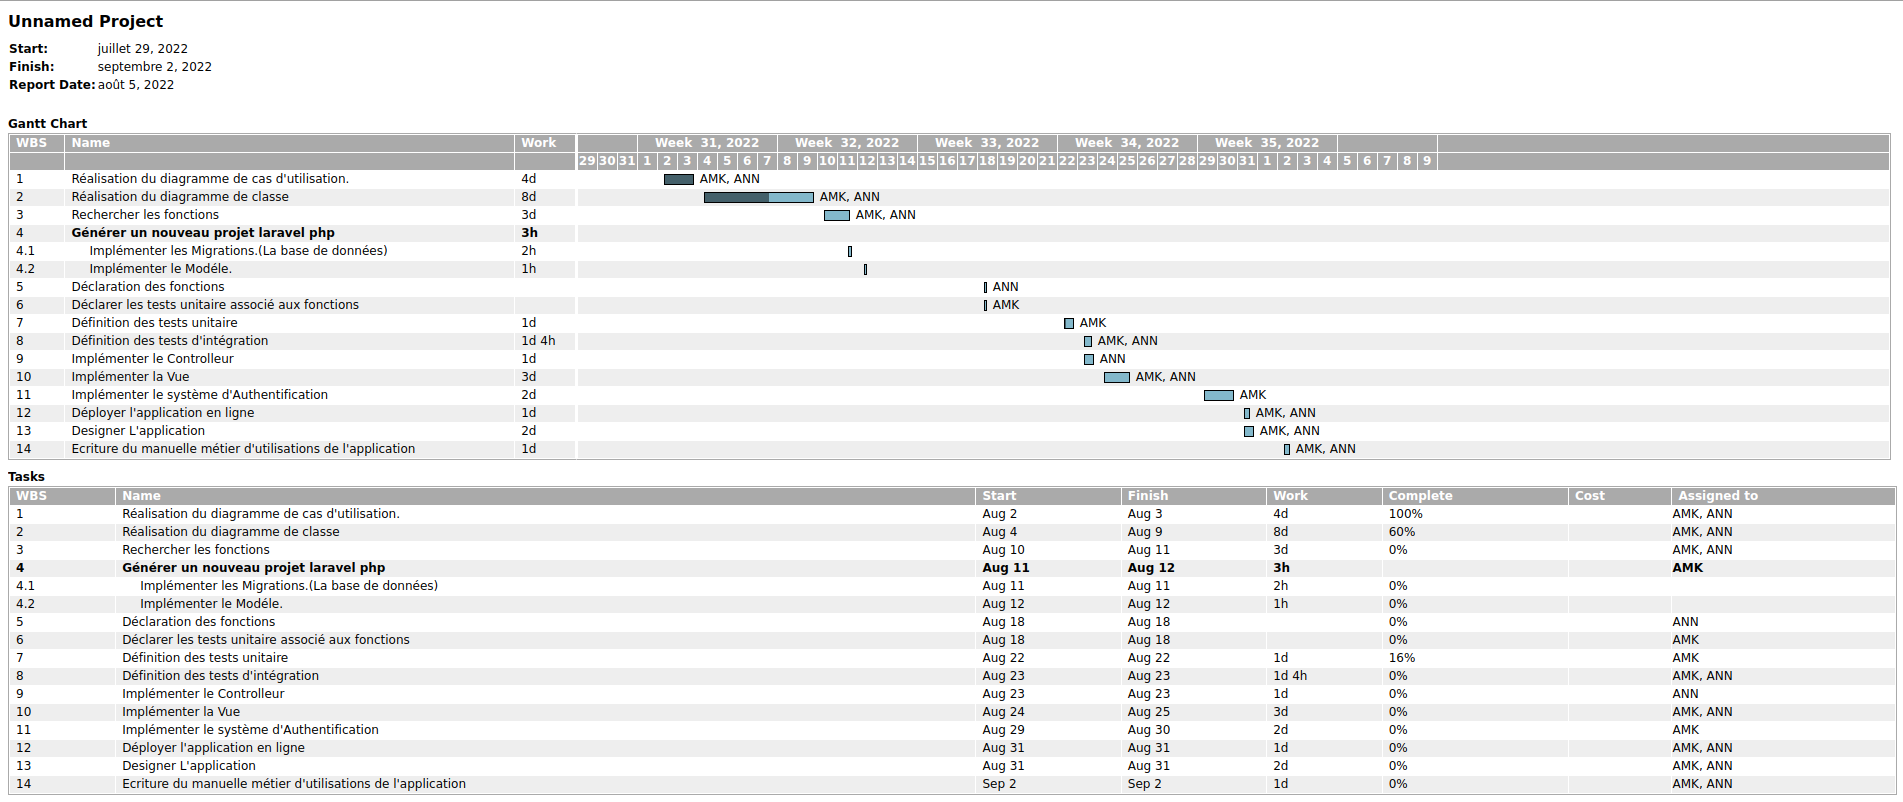
\includegraphics[scale=0.23]{images/jour5.png}
Les activités fait ce vendredi ont été :
\begin{itemize}
\item La mise à jour de notre répertoire de travail sur git.
\item La mise à jour de notre diagramme de gant.
\item La consultation des registres de données chez la bibliothécaire.
\end{itemize}
\section{Conclusion}
	En résumé, cette semaine nous avons réalisé \textbf{75\%} du modèle.\\
	Le modèle était estimé à 10 jours (du 1 août au 12 août 2022 [\textit{prévision réel contrairement au gant affiché erreur technique}]). Mais aujourd'hui nous somme sûr que nous le ferrons en 7 jours (avant le 10 août 2022).

\end{document}




